% !TeX root = ../../main.tex
% chktex-file 13
\section{Technology Stack}\label{section:technology-stack}

Since most of the existing software for \gls{UBII} was written in \gls{JS}\footnote{\gls{JS} is a just-in-time compiled programming language, widely used in web technology. It is a dynamic prototype-based language, which supports object-orientated programming~\cite[43, 47]{ECMAInternational.2018}.} using a web-based architecture, the proposed application was also implemented this way. This has the notable advantage of platform independence. Most modern devices can run web-based software, which means they are also able to run this application. Also, the application is served by a web server, which means the user does not have to install any software onto his device.

A web interface (the \gls{UBII} front end) with some examples, demos, and debugging tools was already implemented\footnote{The front end was initially developed by Sandro Weber and Daniel Dyrda. It also contains some improvements as well as the \gls{VR} examples by the author of this thesis.}. Figure~\ref{fig:ubii-front-end} shows a demo application, which renders a \gls{3D} cube. The proposed experiments are included in this front end, as well.

\begin{figure}[H]
	\centering
	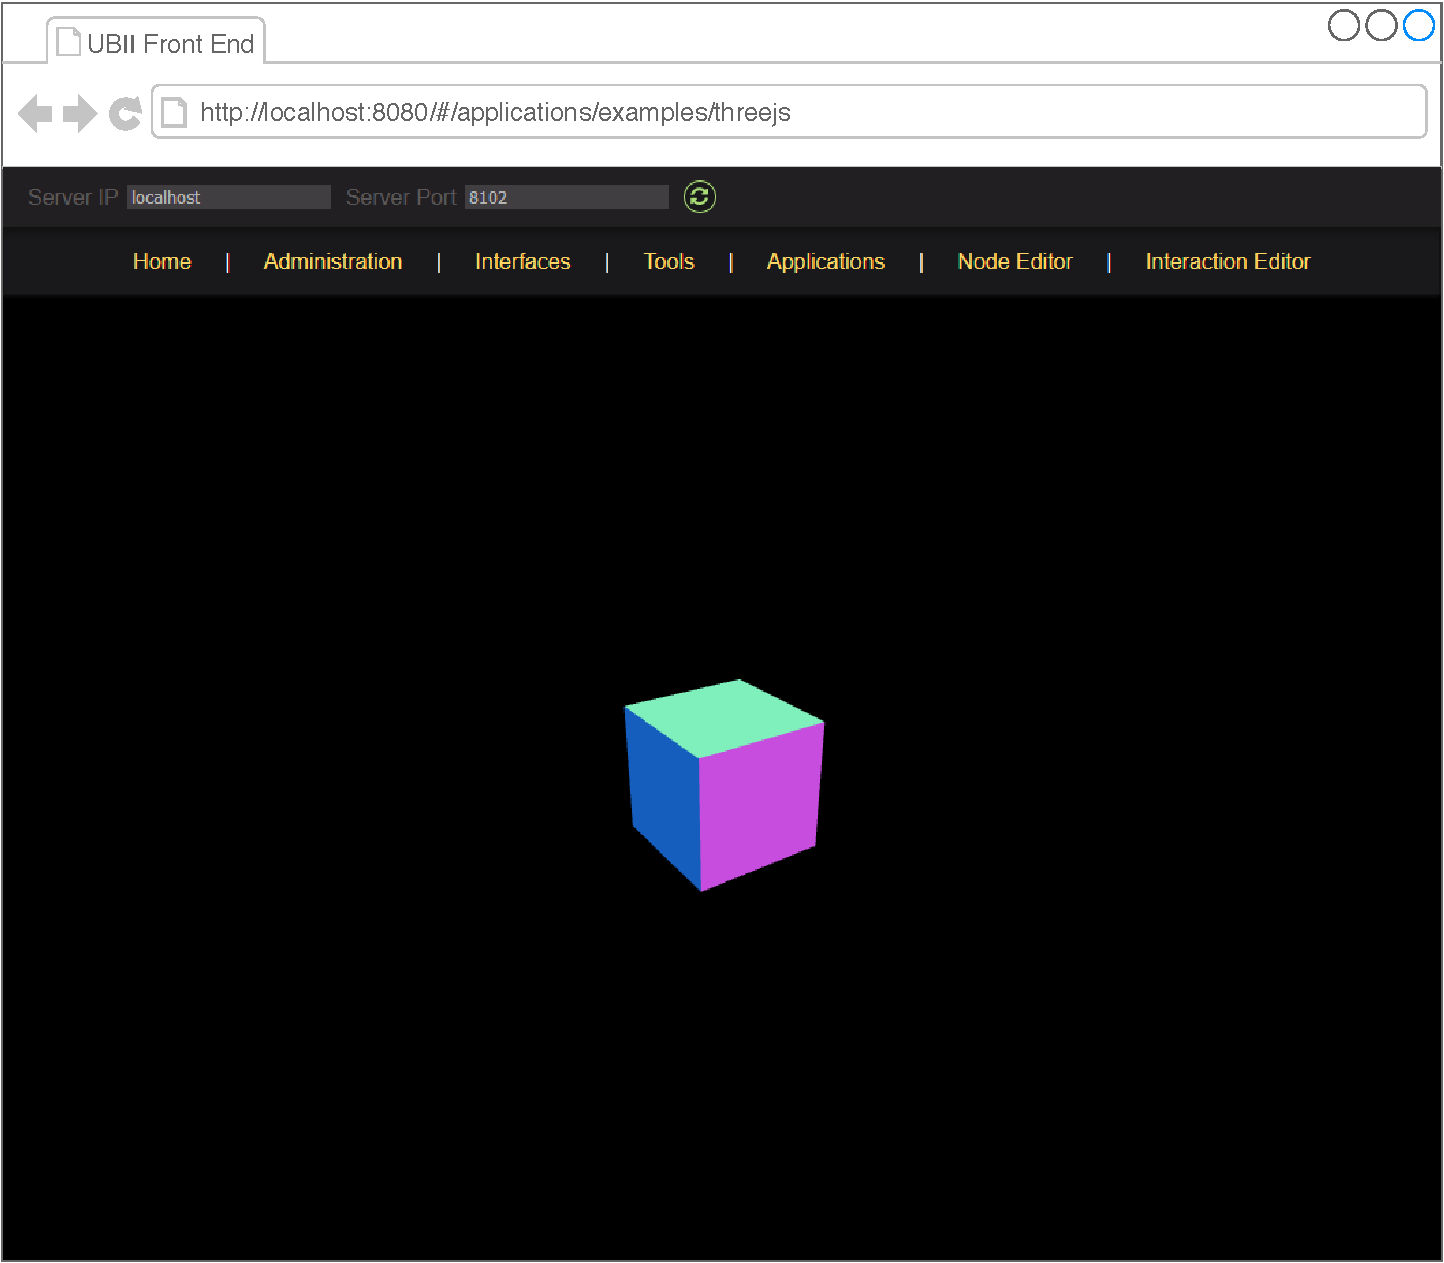
\includegraphics[width=10cm]{figures/implementation/ubii_front_end.pdf}
	\caption[Screenshot of the front end]{A screenshot of a demo application in the UBII front end, rendering a \gls{3D} cube. The bar at the top of the website is displaying the connection data of the currently connected \gls{UBII} server. Below that, the main navigation bar is displayed. It allows to navigate to the applications and tools embedded into the \gls{UBII} front end.}\label{fig:ubii-front-end}
\end{figure}

The technology stack of the front end was built with the following technologies:
\begin{description}
	\item[Web APIs] are \acrlongpl{API} available in modern web browsers to provide access to functionality or data outside the web page. The WebAPI provides an additional layer of abstraction of certain functions of an \gls{OS}. This has the advantage that the API is the same on every device. But in terms of sensors, this prevents the access to the raw sensor data\footnote{The specification is available on \href{https://w3c.github.io/deviceorientation/}{www.w3c.github.io/deviceorientation}}. In this thesis, the WebVR \gls{API} and the device orientation \gls{API} were used. The former enables to render to external \gls{VR} headsets. The latter gives access to the data of the \gls{IMU}.
	 
	\item[Vue.js] is a modern open-source \acrlong{JS} web framework\footnote{A web framework is a software framework which provides a standard way to build web applications. It comes with tools and libraries to automate and make the development of web applications easier.}\footnote{Vue.js: Website: \href{https://vuejs.org/}{www.vuejs.org}; Source~code: \href{https://github.com/vuejs/vue}{www.github.com/vuejs/vue}}~\cite{You.2019}. Being released in 2014 and developed by Evan You, it is a relatively young framework~\cite[17]{Koetsier.2016}. However, it quickly gained traction and is quite popular now~\cite[12\psq]{Koetsier.2016}.
  Packages like Vue.js itself, Vue.js plugins and other \acrlong{JS} libraries are managed using the package manager npm\footnote{\enquote{NPM} stands for \enquote{Node Package Manager} and is also used in the~\gls{UBII} server itself. Website: \href{https://www.npmjs.com/}{www.npmjs.com}}.
  
	\item[Three.js] is a lightweight open-source library which utilizes WebGL to render \gls{3D} computer graphics\footnote{Three.js: Website: \href{https://threejs.org/}{www.threejs.org}, Source~code: \href{https://github.com/mrdoob/three.js/}{www.github.com/mrdoob/three.js}}~\cite{Cabello.2019}. It can be used to render scenes to the display as well as to a \gls{HMD} using WebVR. This high-level library comes with a lot of features, similar to a game engine, like scenes, effects, lights, animation, geometry, and more.
	 
	\item[UBII Client] is an \acrlong{JS} client for the \gls{UBII} system. It abstracts the protocol and provides high-level functions, for example, to register Devices or to send and receive Topic data.
\end{description}

